\documentclass{beamer}

\usetheme{metropolis}

\metroset{
  progressbar=frametitle,   % thin progress bar under each title
  block=fill,
  numbering=fraction        % "3/12" instead of just "3"
}
\usepackage{graphicx}
\title{Case Studies: Sports Analytics}
\author{Nicholas, Sriram, Rohit, Silas}
\begin{document}
    \maketitle
\begin{frame}
    \frametitle{Tennis Classification Tree}

    Highlight of Tennis Grid Search Model Comparison
    \newline
    \resizebox{\textwidth}{!}{
        \begin{tabular}{l|r|r|r|r|r|r}
        \hline
        comment & cp & minsplit & maxdepth & train\_error & test\_error & nsplits\\
        \hline
        least test error & 0.000 & 2 & 1 & 0.229 & 0.277 & 1\\
        \hline
        reasonable performer using more than one split & 0.001 & 40 & 5 & 0.224 & 0.279 & 6\\
        \hline
        worst overfit & 0.000 & 2 & 15 & 0.079 & 0.345 & 434\\
        \hline
        \end{tabular}
    }
    \newline
    \small Winner is a \textbf{single split on elo}: 72.3\% of unseen matches
    correct (logistic regression 73.1\%, coin flip 50\%).
    \newline

    \begin{columns}[c]
        \begin{column}{0.38\textwidth}
            \centering
            \includegraphics[width=\textwidth]{plots/besttree.png}
        \end{column}
        \begin{column}{0.62\textwidth}
            \centering
            \includegraphics[width=\textwidth]{plots/maxdepth_vs_ratio.png}
        \end{column}
    \end{columns}
\end{frame}


\begin{frame}
    \frametitle{Tennis: Why the Tree Stays So Small}

    \begin{columns}[c]
        \begin{column}{0.34\textwidth}
            \small
            \textbf{Default (cp = 0.01)}
            \begin{itemize}
                \item 1 split, uses \texttt{elo} only
                \item only \textbf{2 probabilities}: 0.249 / 0.750
            \end{itemize}
            \vspace{0.4em}

            \textbf{cp = 0.001}
            \begin{itemize}
                \item 22 leaves, \textbf{19 probabilities}
                \item uses \textbf{all four} predictors
            \end{itemize}
        \end{column}
                \begin{column}{0.66\textwidth}
            \centering
            \includegraphics[width=0.63\textwidth]{plots/jitter_boxplot.png}
            \\[0.3em]
            \includegraphics[width=0.63\textwidth]{plots/cp0001boxplot.png}
            \\[0.2em]
            \tiny Predicted winning probabilities by outcome:
            2 values (top, cp = 0.01) vs.\ 19 values (bottom, cp = 0.001).
        \end{column}
    \end{columns}
\end{frame}


    \begin{frame}
        \frametitle{Handball Tree Regression}

        Highlight of Handball Grid Search Model Comparison
        \newline
        \resizebox{\textwidth}{!} {
            \begin{tabular}{l|r|r|r|r|r|r|r|r}
            \hline
            comment & cp & minsplit & maxdepth & train\_mae & train\_rmse & test\_mae & test\_rmse & nsplits\\
            \hline
            best test mae & 0 & 40 & 5 & 3.288 & 4.213 & 3.588 & 4.582 & 25\\
            \hline
            compromise btw number of splits \& test mae & 0 & 2 & 3 & 3.375 & 4.307 & 3.638 & 4.606 & 7\\
            \hline
            worst overfit in mae \& rmse & 0 & 2 & 15 & 0.916 & 1.915 & 4.859 & 6.387 & 914\\
            \hline
            \end{tabular}
        }
        \newline
        \newline

        
        \begin{columns}[c]
            \begin{column}{0.4\textwidth}
                Best compromise: 
                \centering
                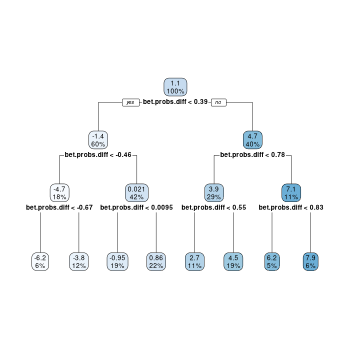
\includegraphics[width=\textwidth]{plots/handball-compromise-rpart-plot.png}
            \end{column}
            \begin{column}{0.6\textwidth}
                \newline
                \centering
                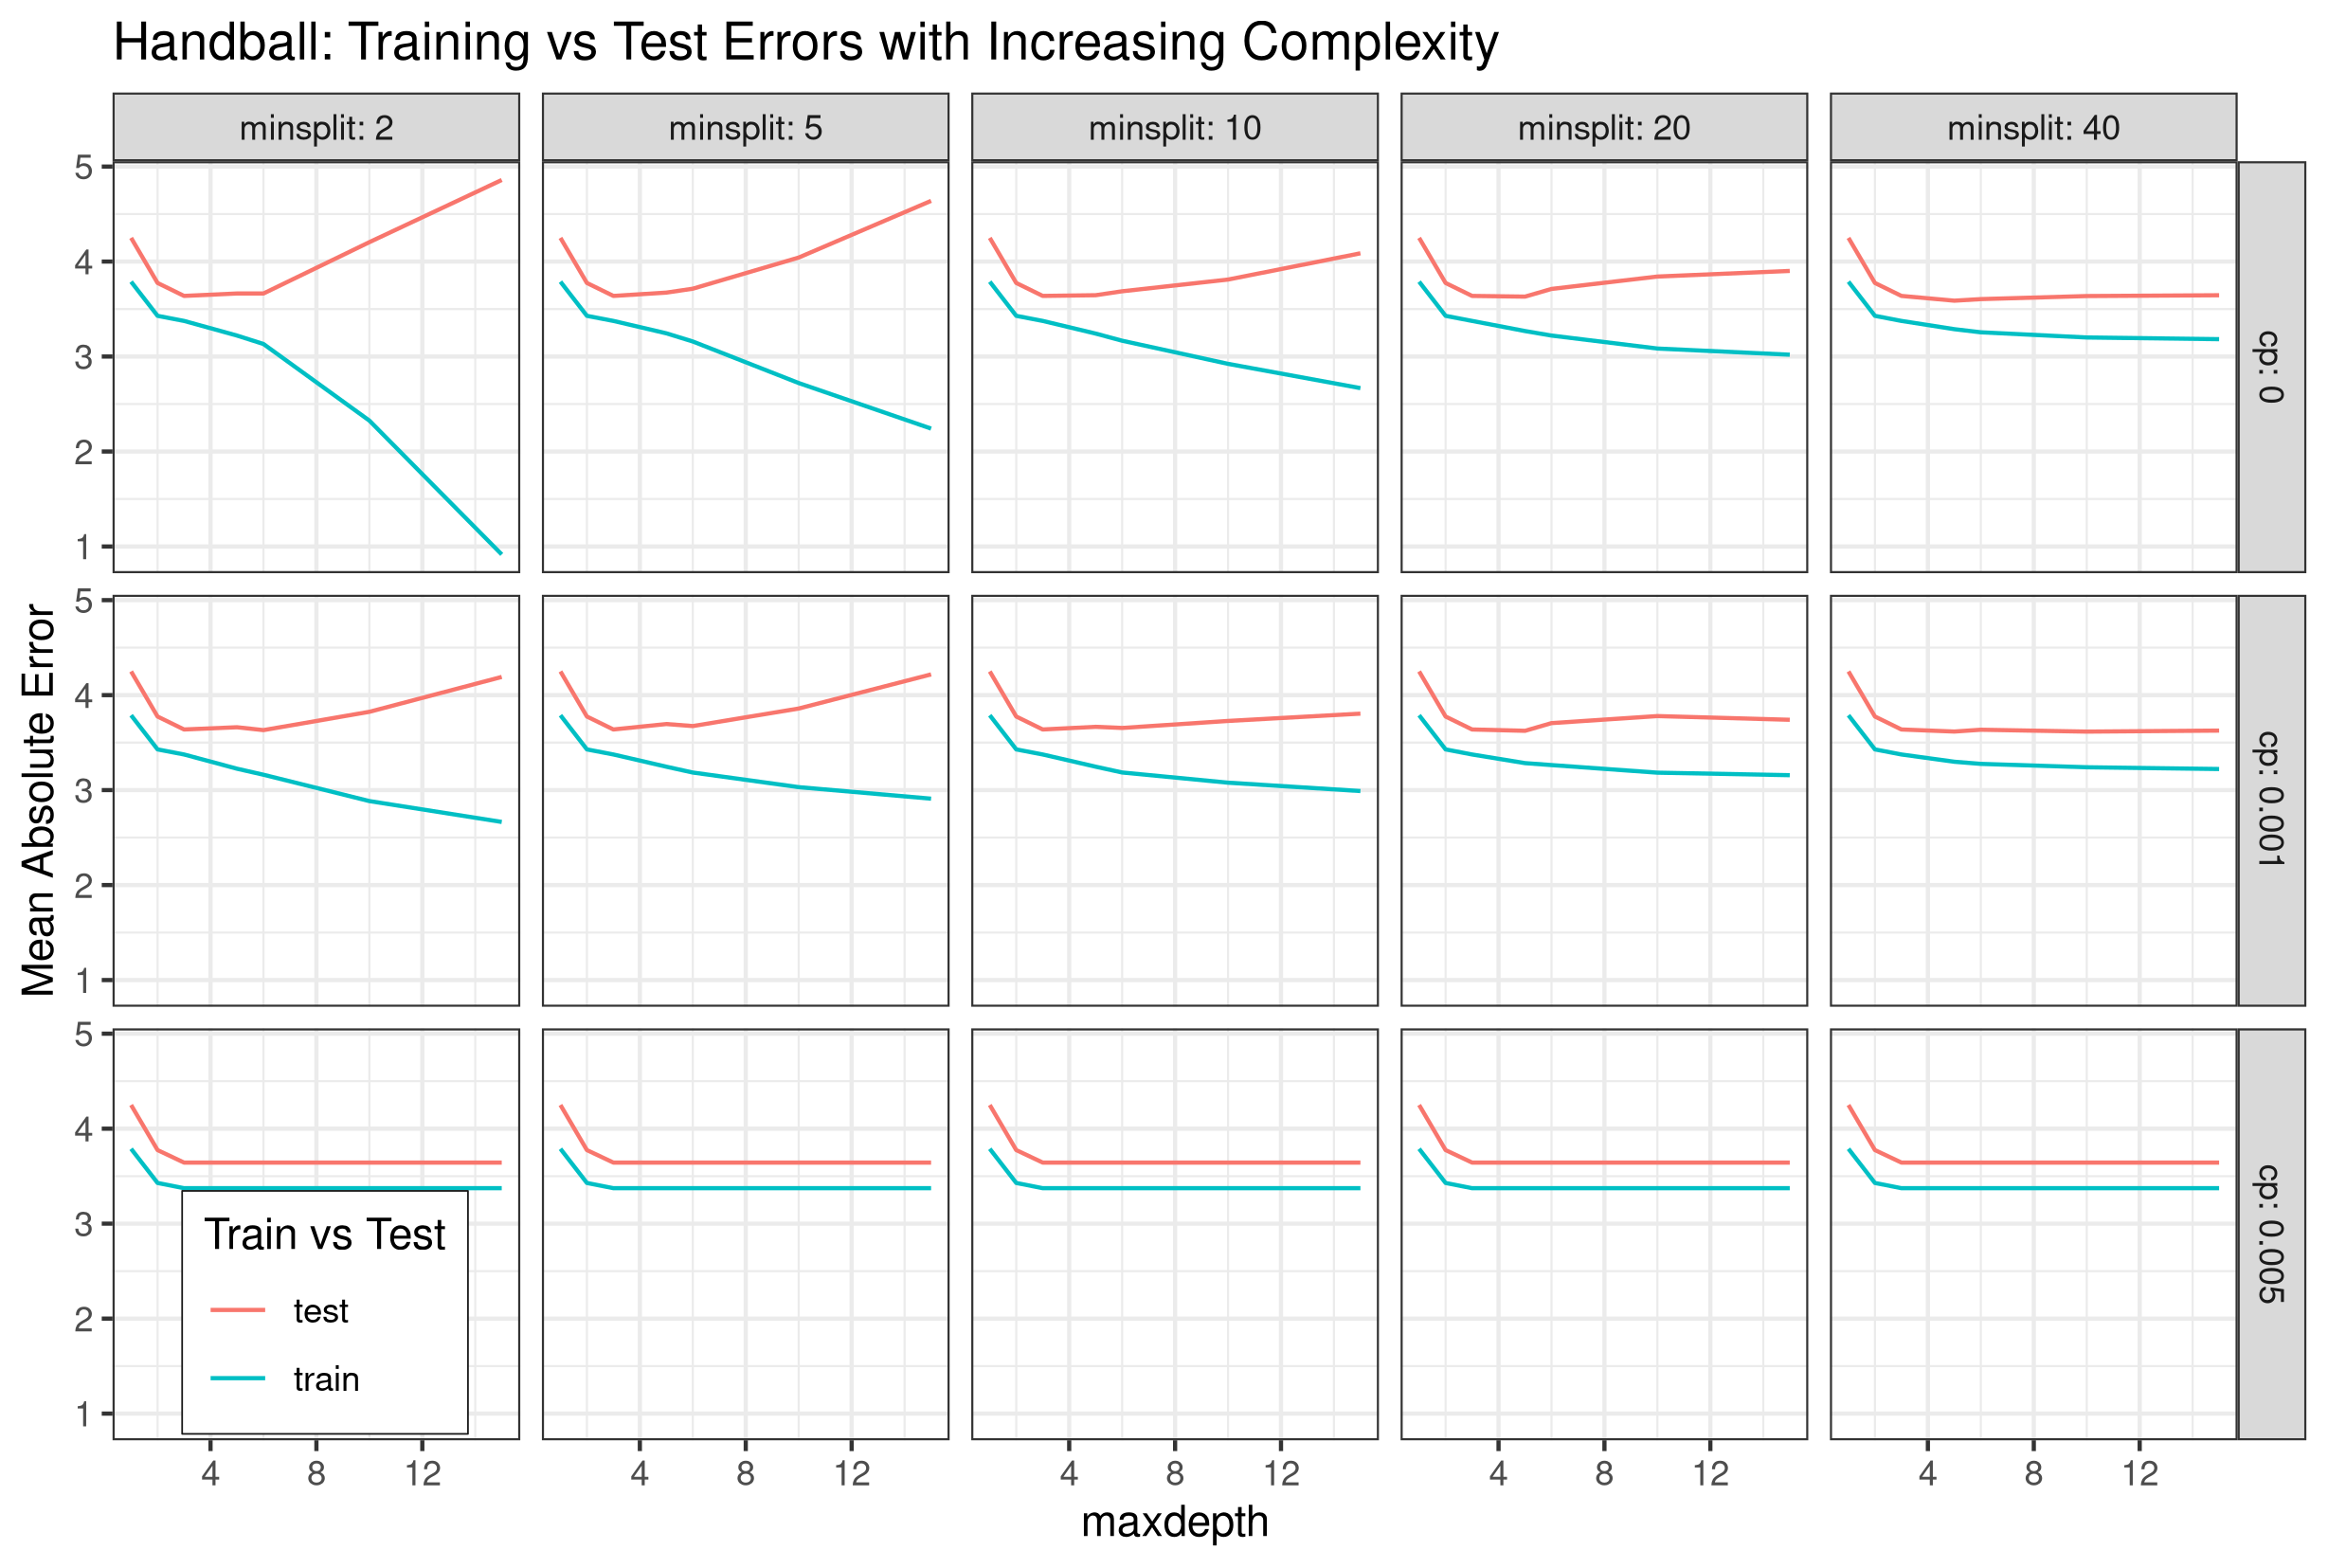
\includegraphics[width=\textwidth]{plots/handball-overfit-complexity-facet.png}
            \end{column}
        \end{columns}
    \end{frame}

\begin{frame}
    \frametitle{Football Regression Trees: Model Selection}

    \centering
    \scriptsize
    \textbf{Tree specifications and predictive performance}

    \vspace{0.1cm}

    \resizebox{0.92\textwidth}{!}{
        \begin{tabular}{l|r|r|r|r|r|r}
            \hline
            Tree & cp & minsplit & maxdepth &
            Train MAE & Test MAE & Test RMSE \\
            \hline
            Baseline tree & 0.01 & 20 & 30 &
            0.779 & 0.784 & 1.055 \\
            Best tree & 0 & 5 & 3 &
            0.780 & 0.741 & 0.985 \\
            Worst overfit tree & 0 & 2 & 15 &
            0.112 & 1.326 & 1.716 \\
            \hline
        \end{tabular}
    }

    \vspace{0.2cm}

    \begin{columns}[T,onlytextwidth]
        \begin{column}{0.49\textwidth}
            \centering
            \textbf{Best regression tree}

            \vspace{0.08cm}
            
\includegraphics[
                width=\linewidth,
                height=0.48\textheight,
                keepaspectratio
            ]{plots/football-best-rpart-plot.png}
        \end{column}

        \begin{column}{0.49\textwidth}
            \centering
            \textbf{Training vs. test error}

            \vspace{0.08cm}
            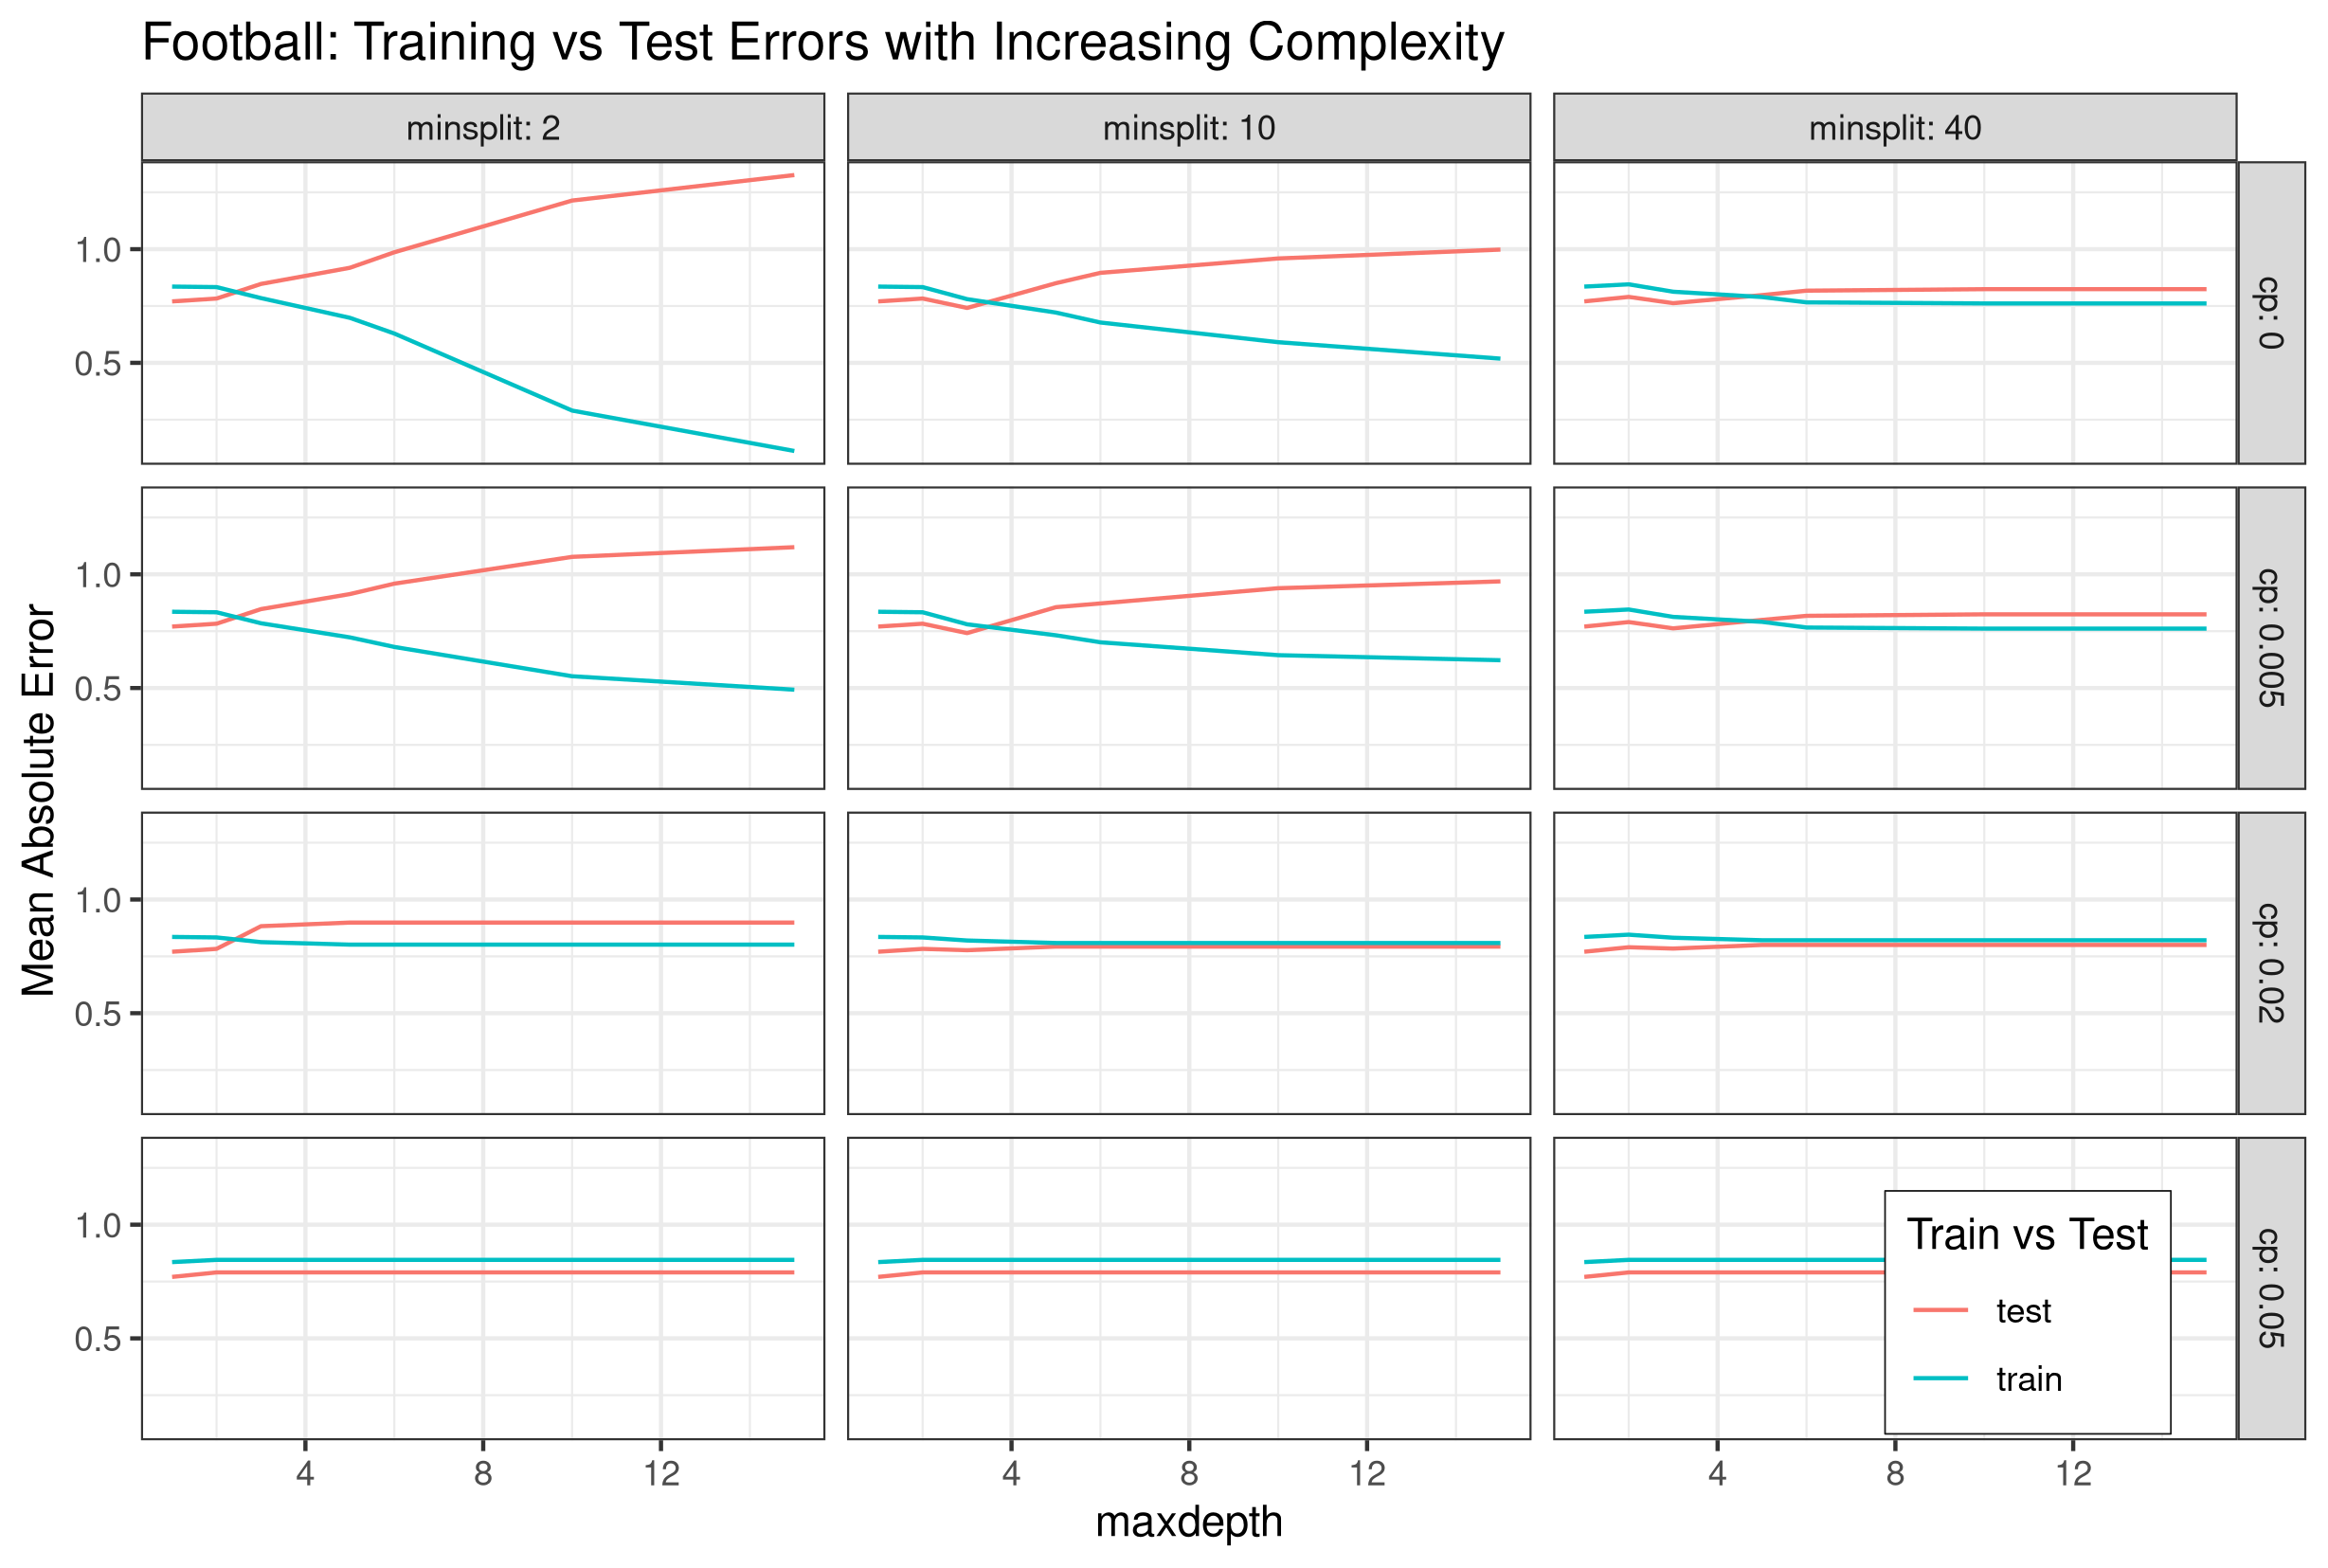
\includegraphics[
                width=\linewidth,
                height=0.48\textheight,
                keepaspectratio
            ]{plots/football-overfit-complexity-facet.png}
        \end{column}
    \end{columns}

\end{frame}

\begin{frame}
    \frametitle{Football Regression Trees: Interpretation}

    \begin{columns}[T,onlytextwidth]
        \begin{column}{0.49\textwidth}
            \centering
            \textbf{Splits based on market value}

            \vspace{0.08cm}
            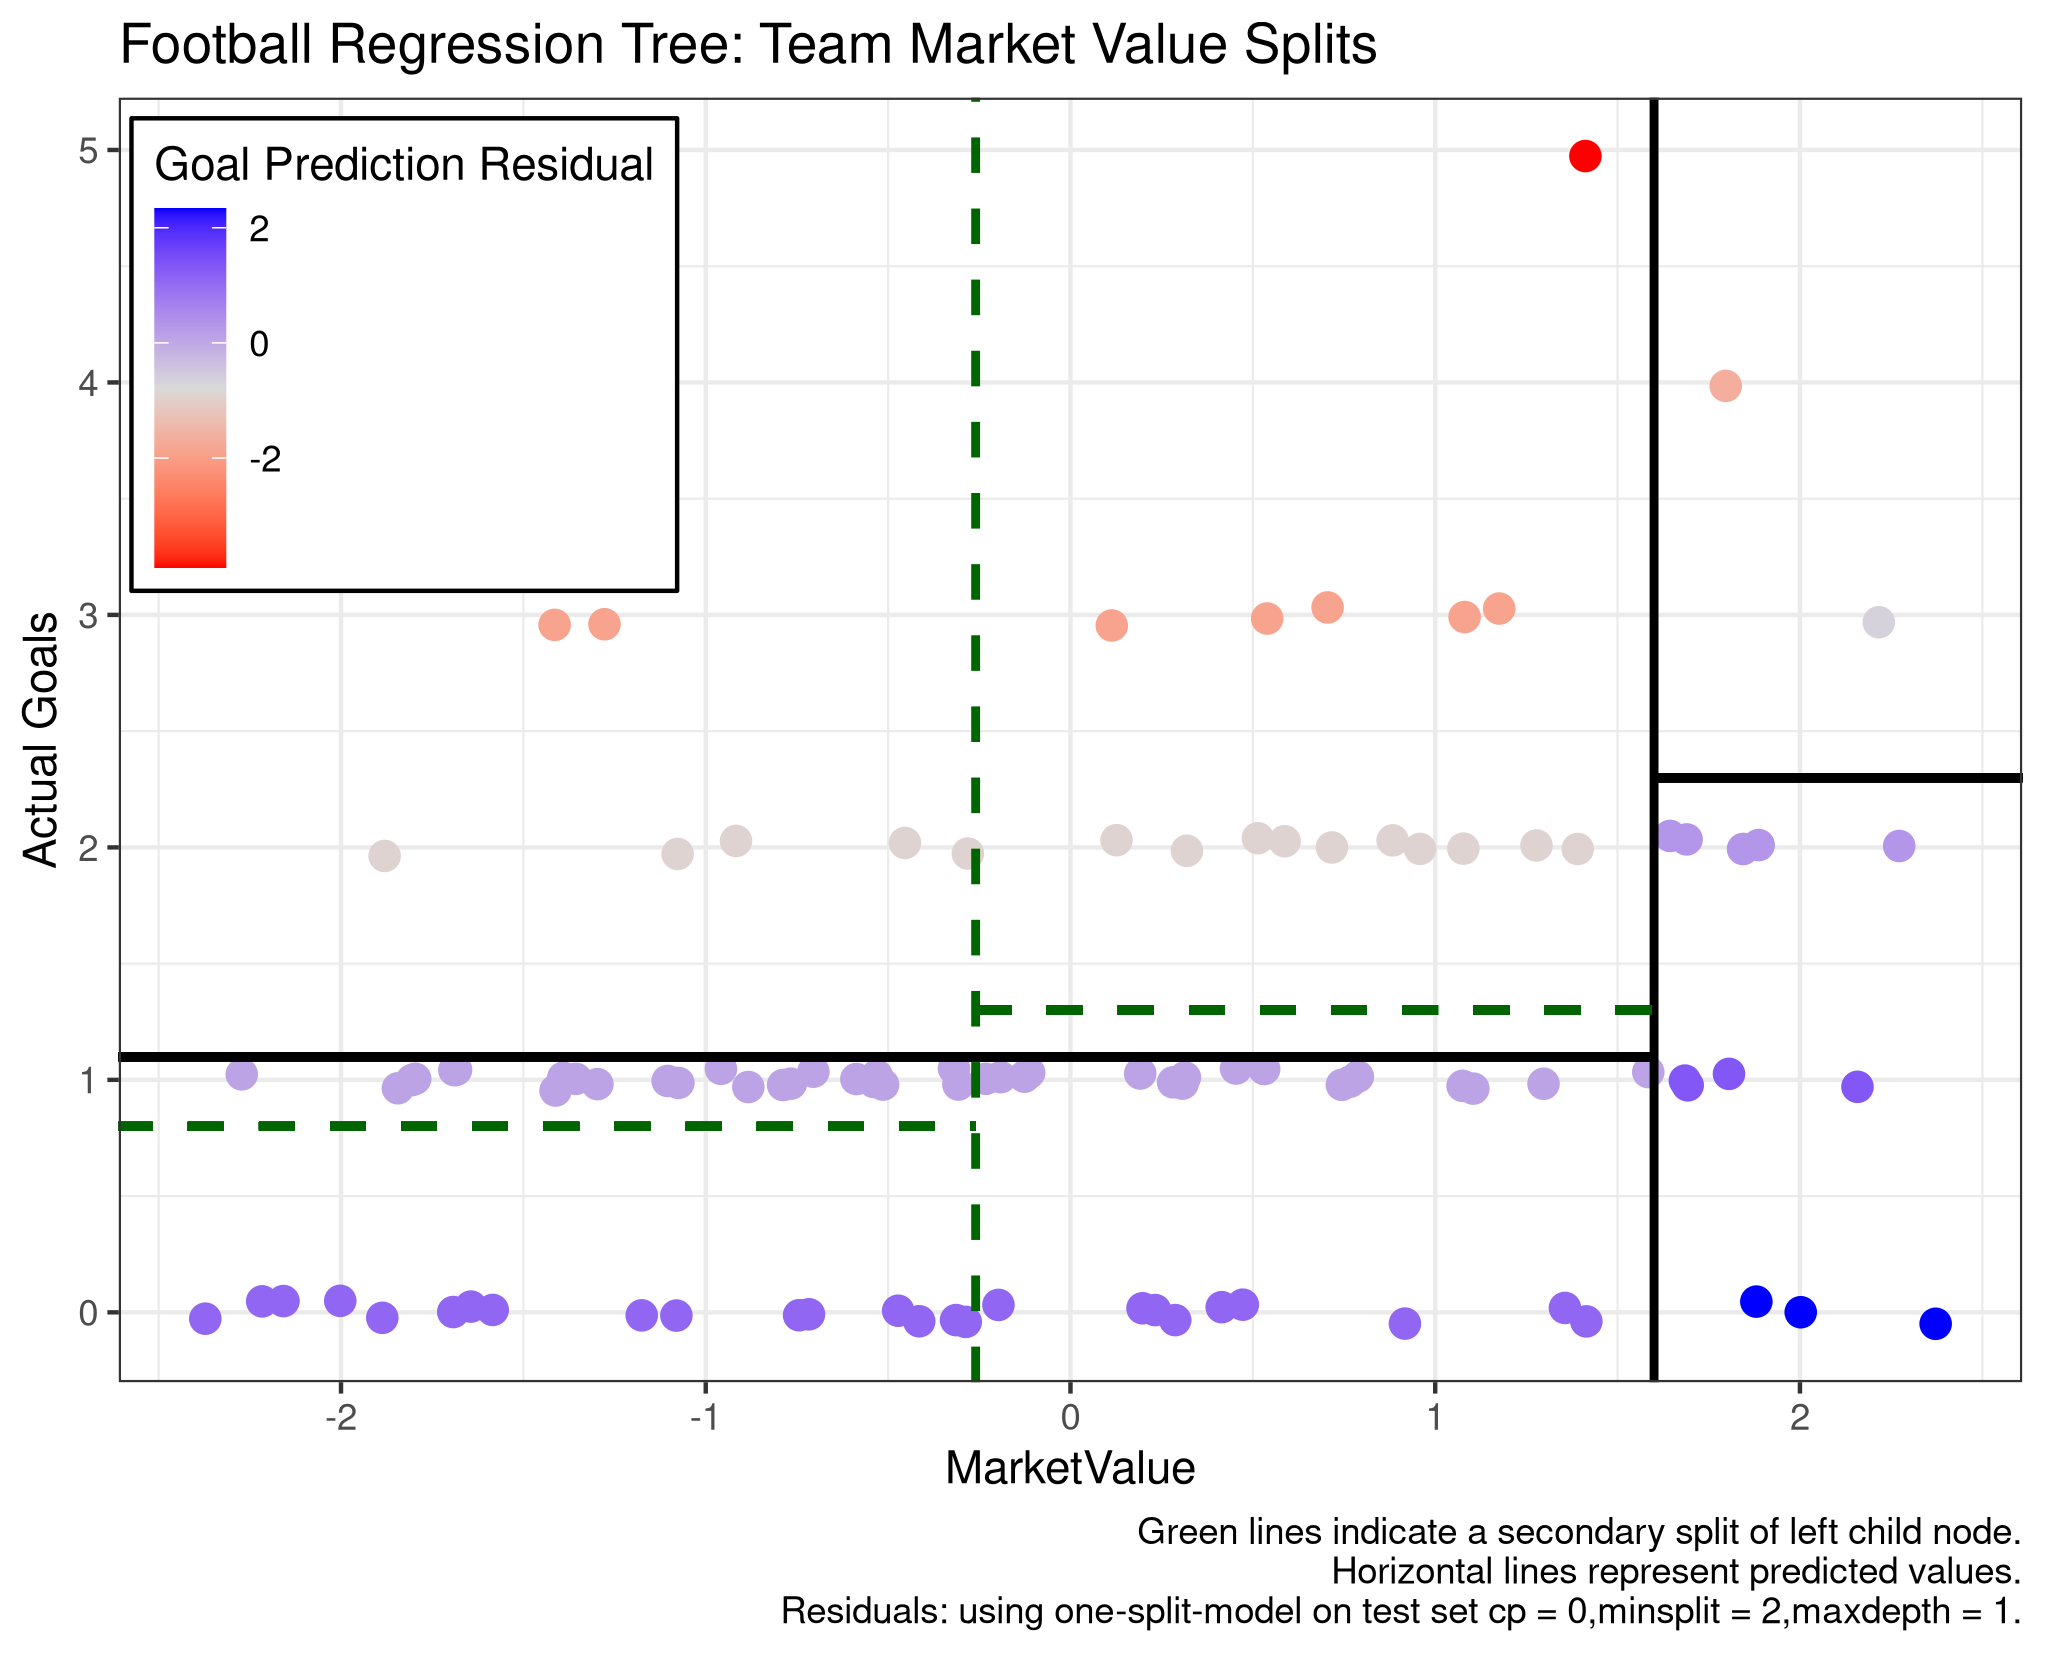
\includegraphics[
                width=\linewidth,
                height=0.5\textheight,
                keepaspectratio
            ]{plots/football-splits-marketvalue.png}
        \end{column}

        \begin{column}{0.49\textwidth}
            \centering
            \textbf{Variable importance}

            \vspace{0.08cm}
            \includegraphics[
                width=\linewidth,
                height=0.5\textheight,
                keepaspectratio
            ]{plots/football-variable-importance.png}
        \end{column}
    \end{columns}

    \vspace{0.3cm}

    \centering
    \scriptsize
    \textbf{Predictive performance on Euro 2024 test data}

    \vspace{0.25cm}

    \begin{tabular}{l|r|r}
        \hline
        Model & Test MAE & Test RMSE \\
        \hline
        Baseline model & 0.781 & 1.006 \\
        Best regression tree & 0.741 & 0.985 \\
        Lasso regression & 0.735 & 0.946 \\
        \hline
    \end{tabular}

    \vspace{0.08cm}

\end{frame}

\end{document}